\documentclass[a4paper,oneside]{thesis}
\usepackage[utf8]{vietnam}
\renewcommand{\rmdefault}{utm}
\renewcommand{\sfdefault}{uhv}
\renewcommand{\ttdefault}{ucr}
\usepackage[unicode,hidelinks]{hyperref}
%\setmathfont{Asana-Math}
\usepackage{fix-cm}
\usepackage{color}
%\usepackage{lyk-z13}
%\usepackage[unicode]{hyperref}
\usepackage{amscd,amssymb}
%\usepackage{array} % Load array package before xy-pic to avoid conflicts
%\usepackage[v2,cmtip]{xy} % Commented out due to conflicts with array package
\usepackage{urwchancal}
\usepackage{amsthm}
\usepackage{rotating}
%%%%%%%%%%%%%%%%%

\usepackage{longfbox}%gGói lệnh đóng khung văn bản đẹp
\usepackage{listings}
\usepackage{mathptmx}
\usepackage{subfig}
\usepackage{colortbl}
\usepackage{graphicx}
\usepackage{array} % Needed for p{...} column types in tabular
\usepackage{multicol}
\usepackage{longtable}
\usepackage{indentfirst}
\usepackage{makeidx}
\usepackage{xspace}
\usepackage{titlesec}
\usepackage{multicol}
%\usepackage{pb-diagram}
\usepackage{titletoc}
%\usepackage{glossaries}
 %\usepackage{maybemath}
%\usepackage{aliascnt}
\usepackage{wallpaper} 
\usepackage{fancybox}
\usepackage {imakeidx}
\input vntypeset_t5_c.tex
%\input diagxy
\newlength{\defbaselineskip}
\setlength{\defbaselineskip}{\baselineskip}
\newcommand{\setlinespacing}[1]%
           {\setlength{\baselineskip}{#1 \defbaselineskip}}
\newcommand{\doublespacing}{\setlength{\baselineskip}%
                           {2.0 \defbaselineskip}}
\newcommand{\singlespacing}{\setlength{\baselineskip}{\defbaselineskip}}
\renewcommand{\sectionmark}[1]{\markright{\small{\textit{\thesection. #1}}}{}}


% Chen code Matlab
\usepackage{listings}
\definecolor{dkgreen}{rgb}{0,0.6,0}
\definecolor{gray}{rgb}{0.5,0.5,0.5}
\definecolor{mauve}{rgb}{0.58,0,0.82}

\lstset{frame=tb,
 language=matlab,
 aboveskip=3mm,
 belowskip=3mm,
 showstringspaces=false,
 columns=flexible,
 basicstyle={\small\ttfamily},
 numbers=none,
 numberstyle=\tiny\color{gray},
 keywordstyle=\color{blue},
 commentstyle=\color{dkgreen},
 stringstyle=\color{mauve},
 breaklines=true,
 breakatwhitespace=true,
 tabsize=3
}
\newtheorem{matlab}{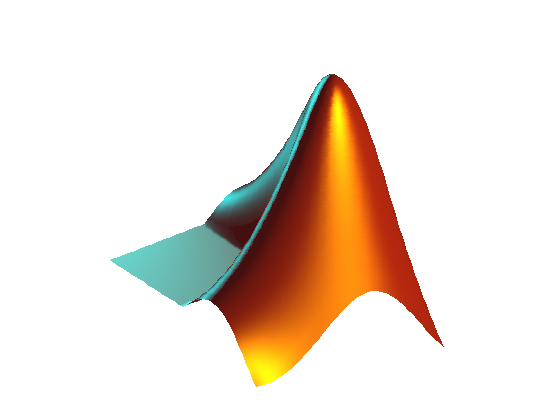
\includegraphics[scale=.11,bb= 500 300 50 250]{logomatlab.png}M.}[chapter]




%%%%%%%%%%%%%



\begin{document}


%%%%%%%%%%%%%%%% BIA 
%\renewcommand{\normalsize}{\fontsize{13}{18}\selectfont}
\fontsize{13pt}{22pt}\selectfont
%\dominitoc
%\pagestyle{myheadings}
%\pagenumbering{arabic}
\ThisCenterWallPaper{1}{frame4.png}

\thispagestyle{empty}
\begin{titlepage}

\hspace{2.8cm} {\bf \fontsize{16pt}{16}\selectfont TRƯỜNG ĐẠI HỌC CẦN THƠ}\\
\vspace*{0.05cm}
\hspace{3.3cm} {\bf\fontsize{16pt}{16}\selectfont KHOA KHOA HỌC TỰ NHIÊN}\\
 \vspace*{0.05cm}
\hspace{4.3cm} {\bf\fontsize{16pt}{16}\selectfont BỘ MÔN TOÁN HỌC}\\

\begin{figure}[h!]
\hspace{5cm} 
\includegraphics[width=40mm]{DHCT.png}
\end{figure}

\vspace*{0.5cm}

\hspace{4cm}{\bf\fontsize{16pt}{20}\selectfont BÀI THU HOẠCH}\\
 \vspace*{0.05cm}\\
\vspace*{2cm}

\begin{center}
 {\bf\fontsize{20pt}{28}\selectfont CHUYÊN ĐỀ THỐNG KÊ NÂNG CAO}   
\end{center}




\vspace*{1.5cm}

\begin{center}
\textbf{Sinh viên thực hiện}\\    
\textbf{TRẦN VĂN LÝ }\\
\textbf{NGÀNH LTXS \& TKTH - Khóa 31}\\
\textbf{MSHV: 001111}
\end{center}



\vspace*{3cm}
\hspace{4.0cm}{\bf \fontsize{16pt}{18}\selectfont CẦN THƠ - NĂM 2025}
\end{titlepage}



\newpage

%%% LOT BIA

\begin{titlepage}

\hspace{2.8cm} {\bf \fontsize{16pt}{16}\selectfont TRƯỜNG ĐẠI HỌC CẦN THƠ}\\
\vspace*{0.05cm}
\hspace{3.3cm} {\bf\fontsize{16pt}{16}\selectfont KHOA KHOA HỌC TỰ NHIÊN}\\
 \vspace*{0.05cm}
\hspace{4.3cm} {\bf\fontsize{16pt}{16}\selectfont BỘ MÔN TOÁN HỌC}\\
\vspace*{0.05cm}
\hspace{5 cm} <><><><><><><><> 


\vspace*{2cm}

\hspace{4cm}{\bf\fontsize{16pt}{20}\selectfont BÀI THU HOẠCH}\\
 \vspace*{0.05cm}\\
\vspace*{2cm}

\begin{center}
 {\bf\fontsize{20pt}{28}\selectfont CHUYÊN ĐỀ THỐNG KÊ NÂNG CAO }   
\end{center}




\vspace*{1.5cm}

\begin{center}
\textbf{Sinh viên thực hiện}\\    
\textbf{TRẦN VĂN LÝ}\\
\textbf{NGÀNH LTXS \& TKTH - Khóa 31}\\
\textbf{MSHV: 001111}
\end{center}



\vspace*{3cm}
\hspace{4.0cm}{\bf \fontsize{16pt}{18}\selectfont CẦN THƠ - NĂM 2025}
\end{titlepage}

%%%%%%%%%%%%%%%%%%%%%%%%%%%%%%%%%%%%
\pagenumbering{roman}
\setlinespacing{1.2}

\tableofcontents % mục lục tự động
\newpage
\addcontentsline{toc}{chapter}{{\bf Danh sách hình vẽ}\rm}
\listoffigures % Danh sách hình vẽ tự động

\newpage
\addcontentsline{toc}{chapter}{{\bf Danh sách bảng}\rm}
\listoftables % Danh sách bảng


\vskip2cm
%\hfill\begin{tabular}{c}
%Hà Nội, 2011\\
%Tác giả,\\[7ex]

%\end{tabular}



%\printindex
%%%%%%%%5

%%%%%%%%%%

\newpage


\lmd
\textbf{1. Lý do chọn đề tài}



\textbf{2. Mục tiêu và phạm vi nghiên cứu}

\textbf{2.1. Mục tiêu nghiên cứu}

\textbf{2.2. Phạm vi nghiên cứu}

\textbf{3. Phương pháp nghiên cứu}



\textbf{4. Cấu trúc của luận văn}



\hspace{.5cm} 
\chapter{Kiến thức chuẩn bị}
\setcounter{page}{1}
\pagenumbering{arabic}
Nội dung này được tham khảo và tổng hợp từ các tài liệu tham khảo \cite{1}, \cite{2} và \cite{5}. 


\section{Mục 1 không có dấu chấm cuối dòng}
\subsection{Tiểu mục 1 không có dấu chấm cuối dòng}

Mỗi đoạn diễn đạt cho mỗi ý bao gồm nhiều câu. Mỗi câu phải đầy đủ cú pháp: S + V + O (nếu có).

Qua đoạn mới phải thụt đầu dòng bằng cách chừa 1 dòng trống trong Latex. Thông thường người ta rất hạn chế sử dụng $\setminus\setminus$ để xuống dòng. 
\begin{dn}
 Nội dung định nghĩa viết vào đây
\end{dn}

\[ \int_{x=0}^5 f_X (x) {\rm d}x=1 \]

\begin{dn}
 Nội dung định nghĩa viết vào đây có thể sửa lại
\end{dn}

\begin{dl}
 Nội dung định lý viết vào đây   
\end{dl}

\cm{
Nội dung CM viết vào đây.
}

\subsection{Tiểu mục 2}
%%%%%%%%%Chèn bảng

\begin{table}[ht]
 \caption{\textbf{Bảng minh họa 1}}
    \centering
    \begin{tabular}{|c|c|c|c|c|}
    \hline
     STT    & Họ và tên & Kiểm tra & Thi & Tổng\\
      \hline
     1    & Nguyễn Văn A &  &  & \\
      \hline
      2   &  &  &  & \\
       \hline
         &  &  &  & \\
       \hline
    \end{tabular} 
    %\label{tab:my_label}
\end{table}

%%%%%%%%%%%%%Dạng tùy chỉnh kích thước cột
\begin{table}[ht]
 \caption{\textbf{Bảng minh họa 2}}
 \centering
\begin{tabular}{|c|l|l|l|c|c|}
		\hline
		\textbf{Stt} &\textbf{Tên bài báo} & \textbf{Tác giả/nhóm tác giả}
		& \textbf{Tên tạp chí} &\textbf{Số tạp chí} & \textbf{Năm xuất bản}
		\\
		\hline
		1 &   &  & &  & \\
		\hline
	2 &   &  & &  & \\
		\hline
        3 &   &  & &  & \\
		\hline
	\end{tabular}
    \end{table}
%%%%%%%%%%%%%%%%%%%%%%%%%%%%%%%%%%%%%%%%%%%%%%%%%%
% nội dung này có thể tham khảo giáo trình ĐSTT và HH2
\section{Mục 2}
\subsection{Tiểu mục 1}

\subsection{Tiểu mục 2}

%%%%%%%%%%%%%%%%%%%%%%%%%%%%%%%%%%
\chapter{Một số dạng kiểm định thống kê}





\section{Kiểm đinh Pearson}
\subsection{Hàm phân phối tích luỹ}
\begin{dn}
 Nội dung định nghĩa viết vào đây
\end{dn}

\begin{equation}
    F(x) = P(X<x), \; \forall x \in \mathbb{R}
\end{equation}

\begin{matlab}
\begin{lstlisting}

function [chi_P, chi_J] = pearson_test_V2(N,n)

    % Random variables
    Z = [1 2 3 4 5];

    % Probability corresponding
    PZ = [0.06 0.23 0.35 0.27 0.09];

    % cho nhich len 0.01 de khong cham dau mut
    z = [0 1 1.01 2 2.01 3 3.01 4 4.01 5 5.01 6];

    % Cummulative
    Fz = [0 0 .06 .06 .29 .29 .64 .64 .91 .91 1 1];

    % Lay mau ngau nhien
    sample = randsrc(1,N,[Z; PZ]); % tuy chon so luong mau N ra vi tri xac suat 
    [nz,cz] = hist(sample,n); % phan lam n hop 
    % Tan suat
    fz = nz/N;
    CDFz = cumsum(fz);

    % Tinh toan kiem dinh Pearson
    % Cac tan so ly thuet
    Ei =  PZ*N;

    % Tieu chuan kiem dinh
    chi_P = sum( ((nz - Ei).^2) ./ Ei );

    % Tra gia tri toi han
    chi_J = chi2inv(.95, n - 1);

    subplot(1,2,1)
    % Bieu dien pdf
    plot(Z, PZ, 'r','LineWidth',2)
    hold on

    % 
    bar(cz, fz, 'b')
    hold on
    axis([0 6 0 0.5]) % xac dinh bien do ve

    subplot(1,2,2)
    % Bieu dien CDF Fz
    plot(z,Fz,'r','LineWidth',2) % CDF cua mo hinh
    hold on
    plot(cz,CDFz,'b','LineWidth',1) % CDF cua mo hinh CDFz
    hold off
    axis([0 6 0 1.2]) % xac dinh bien do ve
    figure(1)
end

\end{lstlisting}
\end{matlab}



\begin{figure}[h!]
    \centering
    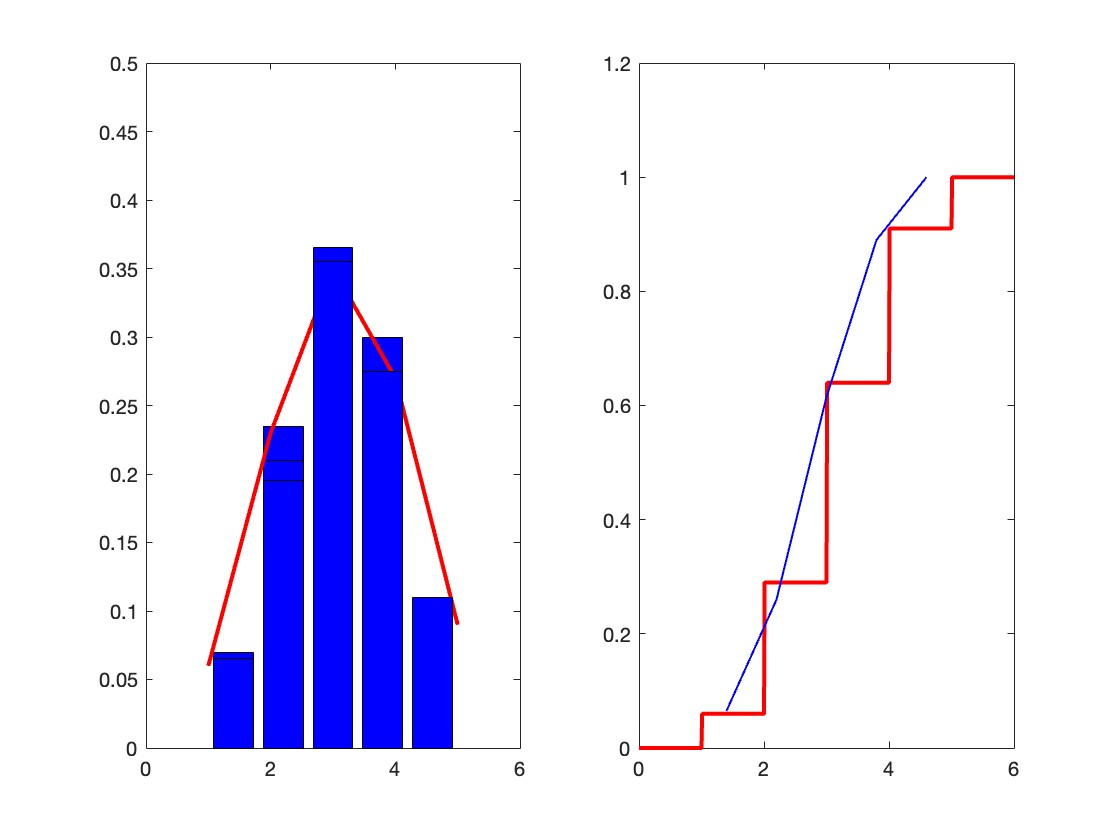
\includegraphics[width=1\linewidth]{image1.jpg}
    \caption{Hình minh họa 1}
    \label{fig:image1-matlab}
\end{figure}


\begin{matlab}
    \begin{lstlisting}
function Ngocppmohinh(c,j1,j2)
    %UNTITLED Summary of this function goes here
    % Version: 1.0
    %  Date: 10/09/24

    % So tham so
    numpara=j2-j1+1;
    % Dat cac tham so ban dau
    xmin=0; xmax=20; ymin=0; ymax=numpara*4;

    % Import the data
    singletons = readtable("singletons.xlsx");


    % Ve cac doi tuong thanh phan

    for i=1:numpara
    % Ve cac nut tren
    plot((xmin+xmax)/2,ymax-4*(i-1),'ob');
    hold on
    % Ve cac vi tri trang thai
        % tim vi tri cac hang trang thai cua tham so i
        hi=find([singletons{:,2}]==j1+i-1);
        % so trang thai thu i
        ni=length(hi);
        % so gia chia deu chieu ngang x
        dx=(xmax-xmin)/(ni+1);
        % vecto cac diem chia deu chieu ngang x
        x=xmin:dx:xmax;
        % Ve cac duong che ra
        % Vong lap cho tung trang thai
        for t=1:ni
        % Ve cac duong che ra
        plot([x(t+1) (xmin+xmax)/2],[ymax-4*(i-1)-2 ymax-4*(i-1)],'-r');
        hold on
        % Ve cac nut
        plot(x(t+1),ymax-4*(i-1)-2,'ob');
        hold on
        % Chen cac ten trang thai
        text(x(t+1)+.4,ymax-4*(i-1)-2-.4,singletons{hi(t),1});
        % Chen cac duong hoi tu
        plot([x(t+1) (xmin+xmax)/2],[ymax-4*(i-1)-2 ymax-4*(i-1)-4],'-r');
        hold on
        % Chen xac suat
        text(x(t+1)-.9, ymax-4*(i-1)-2+.4, [num2str(singletons{hi(t),5})]);
        end % t=1:ni
    end % for i=1:numpara

        % Ve nut ket thuc
        plot((xmin+xmax)/2,ymin,'ob');
        hold off
        
        % Chen cac 
        title('Graph of the clique Singletons')
        axis([xmin xmax ymin ymax+1])
        
        
        % Ve he truc hoac khong
        if c==0
            axis off
        else
            grid
        end % if c==0
        figure(1)

end % for function
    \end{lstlisting}
\end{matlab}

\begin{dl}
 Nội dung định lý viết vào đây   
\end{dl}

\cm{
Nội dung CM viết vào đây.
}

\begin{tc}
    
\end{tc}

\begin{md}
    
\end{md}

\begin{cy}
    
\end{cy}

\begin{vd}
    
\end{vd}

\begin{nx}
    
\end{nx}

\begin{bd}
    
\end{bd}
\subsection{Tiểu mục 2}
\begin{figure}[h!]
    \centering
    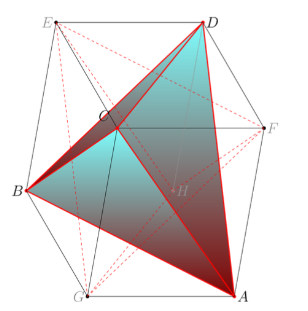
\includegraphics[width=0.3\linewidth]{Hinh1.png}
    \caption{Hình minh họa 1}
    \label{fig:enter-label}
\end{figure}
%%%%%%%%%%%%%%%%%%%%%%%%%%%%%%%%%%%%%%%%%%%%%%%%%%
% nội dung này có thể tham khảo giáo trình ĐSTT và HH2
\section{Mục 2}
\subsection{Tiểu mục 1}

\subsection{Tiểu mục 2}



%%%%%%%%%%%%%%%%%%%%%%%%%%%%%%%%%%
\chapter{Phân tích nhiều chiều dữ liệu thang đo định lượng}


Nội dung này được tham khảo và tổng hợp từ các tài liệu tham khảo  .....

\section{Kiem dinh Pearson}
\subsection{Ham phan phoi tich luy}
\begin{equation}
    F(x) = P(X<x)
\end{equation}
% Mỗi hình một caption
\begin{figure}[h]
    \centering
    % Hình thứ nhất
    \begin{minipage}{0.45\textwidth}
        \centering
        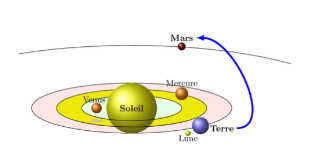
\includegraphics[width=\textwidth]{Hinh2.png}
        \caption{Hình 1}
        \label{fig:image1}
    \end{minipage}
    \hfill
    % Hình thứ hai
    \begin{minipage}{0.45\textwidth}
        \centering
        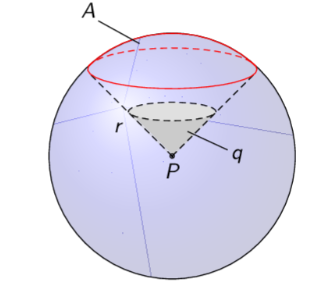
\includegraphics[width=0.7\textwidth]{Hinh3.png}
        \caption{Hình 2}
        \label{fig:image2}
    \end{minipage}
\end{figure}

% Hai hình 1 caption

\begin{figure}[h]
    \centering
    % Hình thứ nhất
    \begin{minipage}{0.45\textwidth}
        \centering
        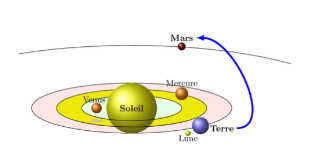
\includegraphics[width=\textwidth]{Hinh2.png}
          \end{minipage}
    \hfill
    % Hình thứ hai
    \begin{minipage}{0.45\textwidth}
        \centering
        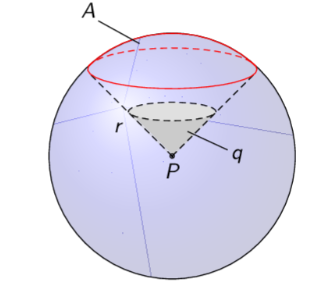
\includegraphics[width=0.7\textwidth]{Hinh3.png}
    \end{minipage}
    \caption{Hình đôi}
        \label{fig:image3}
\end{figure}
\subsection{Tiểu mục 2}

%%%%%%%%%%%%%%%%%%%%%%%%%%%%%%%%%%%%%%%%%%%%%%%%%%
% nội dung này có thể tham khảo giáo trình ĐSTT và HH2
\section{Mục 2}
\subsection{Tiểu mục 1}

\subsection{Tiểu mục 2}

\noindent % Để loại bỏ thụt lề đầu dòng
\begin{minipage}{0.4\textwidth} % Phần hình ảnh (40% chiều rộng trang)
    \centering
    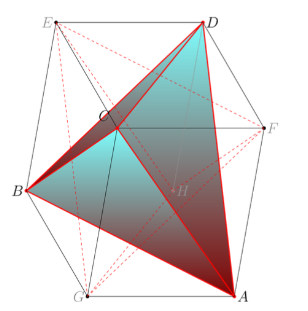
\includegraphics[width=\textwidth]{Hinh1.png} % Đường dẫn tới ảnh
    \captionof{figure}{Hình minh họa} % Chú thích cho hình
    \label{fig:image}
\end{minipage}%
\hfill % Thêm khoảng cách giữa hình và chữ
\begin{minipage}{0.55\textwidth} % Phần văn bản (55% chiều rộng trang)
    Đây là đoạn văn bản mô tả hình ảnh. Bạn có thể viết bất kỳ nội dung nào ở đây để giải thích hoặc chú thích cho hình bên cạnh. Sử dụng phần trăm chiều rộng hợp lý để tối ưu bố cục tài liệu.
\end{minipage}
%%%%%%%%%%%%%%%%%%%%%%%%%%%%%%%%%%


\chapter*{KẾT LUẬN}
\addcontentsline{toc}{chapter}{KẾT LUẬN}


\begin{thebibliography}{70}
\section*{\hskip-\leftmargin Tiếng Việt}
\bibitem{1} Nguyễn Văn A (1999). \textit{Tên sách in nghiêng}, Tên NXB.
\bibitem{2} Nguyễn Văn B và Trần Thị C (1982). Tên bài báo, \textit{Tên tạp chí in nghiêng}, Số xuất bản, Trang 11--20.
\bibitem{3} Nguyễn Văn C (2022). \textit{Tên luận văn in nghiêng}, Luận văn Thạc sĩ hay Đại học, Tên Trường Đại học.



\section*{\hskip-\leftmargin Tiếng Anh}
\bibitem{4} D. Alibaba (1982). \textit{The tittle of book}, Publishing House.
\bibitem{5} F. Colony (2006). The tittle of paper, \textit{Journal's name}, Vol. xx, page 11--20.
\bibitem{} E. Marcos (2024). \textit{Thesis's tittle}, Master's thesis or Bachelor's thesis, Bonba University.
%\bibitem{8} 

 
\end{thebibliography}

%HƯỚNG DẪN CÁCH GHI TLTK XÓA BỎ KHI HOÀN THANH LUẬN VĂN
\begin{table*}
\centering
\begin{tabular}{|l|l|l|}
    \hline
      Loại trích dẫn   & Trích dẫn trong ngoặc đơn (Parenthetical citation) & Trích dẫn trong câu 
(Narrative citation)
\\
     \hline
       \textbf{Một tác giả}
       
Ghi tác giả và năm
  & (Hường, 2013)
  
(Tain, 1999)
 & Hường (2013)
 
Tain (1999)
\\
    \hline
   \textbf{Hai tác giả}
   
Ghi hai tác giả và năm		
      & (Deharveng $\&$ Bedos, 2000) 
      
(Hồ $\&$ Lư, 2003) & Deharveng and Bedos (2000)

Hồ và Lư (2003)\\
         \hline
       \textbf{Ba tác giả trở lên}
       
Ghi tác giả đầu tiên, theo sau là ``và ctv.'' hoặc ``et al.'' và năm 
  & (Aron et al., 2019)
  
(Hiền và ctv., 2016)

*``và ctv.'', ``et al.'' không viết in nghiêng
 & Aron et al. (2019)
 
Hiền và ctv. (2016)
\\
\hline
  \textbf{Tác giả là một cơ quan, tổ chức}
  
Ghi tên cơ quan và năm (Tên cơ quan có thể viết tắt nếu được trích dẫn hơn một lần trong bài)
       &  (United States Government Accountability Office, 2019)

*Trích dẫn lần đầu:
 (Food and Agriculture Organization of the United Nations [FAO], 1977)
 
*Trích dẫn lần sau:
(FAO, 1977)
 & United States Government Accountability Office (2019)

*Trích dẫn lần đầu:
Food and Agriculture Organization of the United Nations (FAO, 2020)

*Trích dẫn lần sau:
FAO (1977)
 \\
      \hline
       \textbf{Nhiều tài liệu}
       
Sắp xếp các tài liệu theo năm xuất bản tăng dần. Nếu các tài liệu có cùng năm xuất bản, thì sắp xếp theo thứ tự bảng chữ cái.
  & (Hồng và ctv. 2014; Hiền và ctv., 2016; Bộ Giáo dục và Đào tạo, 2017; Cảnh, 2017; Aron, 2019; Belcher, 2019)
  
  *Mỗi tài liệu cách nhau bằng dấu chấm phẩy 
  & Hồng và ctv. (2014), Hiền và ctv. (2016), Bộ Giáo dục và Đào tạo (2017), Cảnh 92017), Aron (2019) và Belcher (2019) \\
         \hline
     \textbf{Nhiều tài liệu cùng cách trích dẫn tác giả}
     
Ghi tác giả và các năm theo thứ tự tăng dần
    & (Vuong et al., 2018, 2019b)

(Cảnh, 2017, 2020)
 & Vuong et al. (2018, 2019b)

Cảnh (2017, 2020)
 \\
         \hline
  \textbf{Nhiều tài liệu cùng cách trích dẫn tác giả và cùng năm xuất bản}
  
Ghi tác giả và năm kèm theo chữ cái a, b, c,$\cdots$ & (Vuong et al., 2019a, 2019b)

(Thanh và ctv., 2021a, 2021b)
 & Vuong et al. (2019a, 2019b)

Thanh và ctv. (2021a, 2021b)
\\
         \hline
      \textbf{Trích dẫn từ nguồn thứ cấp}
      
Ghi tác giả và năm (nếu có) của tài liệu gốc kèm “trích dẫn bởi” hoặc “as cited in” tác giả và năm của tài liệu thứ cấp
   & (Garrison, 2011, as cited in Kattoua et al., 2016)

(Hinh và ctv., 2003, trích dẫn bởi Tuấn $\&$ Minh, 2015)

*Trong danh mục TLTK chỉ liệt kê tài liệu thứ cấp (Kattoua et al., 2016; Tuấn $\&$ Minh, 2015)
 & Garrison (2011, as cited in Kattoua et al., 2016) 

Hinh và ctv. (2013, trích dẫn bởi Tuấn $\&$ Minh, 2015)
\\
        \hline
  \end{tabular}
\end{table*}
%%%%%%%%%%%%%%%%%%%%%%%%%%%%%%%%%%%%%%%%%%%%%%%%%
 \begin{table*}
\centering
\begin{tabular}{|l|l|l|}
    \hline
      Loại trích dẫn   & Trích dẫn trong ngoặc đơn (Parenthetical citation) & Trích dẫn trong câu 
(Narrative citation)
\\
     \hline       
     \textbf{Trích dẫn nguyên văn}
     
Ghi tác giả, năm và trang viết.



Đoạn trích dưới 40 từ: để trong ngoặc kép.
Đoạn trích trên 40 từ: viết riêng đoạn mới, lùi đầu dòng, không dấu ngoặc kép.
    & ``Riêng hai tiếng Cần Thơ trong sử không có ghi chép rõ ràng như các tỉnh khác'' (Minh, 1966, trích dẫn bởi Cảnh, 2020, tr. 232). 


Nguồn gốc tên gọi ``Cần Thơ'' do dân gian truyền lại như sau:

Tương truyền lúc chúa Nguyễn Ánh trên đường bôn tẩu vào Nam đã đi qua nhiều nơi để tránh Tây Sơn mưu đồ phục quốc. Lúc bấy giờ Ngài ngự trên một chiếc thuyền đi ngang dòng sông Hậu, thuộc địa phận huyện Phong Phú thả thuyền theo sóng gió lênh đênh trên mặt nước, bỗng nghe tiếng ngâm thơ, đàn địch, hò hát, hòa nhau rất nhịp nhàng. Ngài xúc động và đặt tên con sông này là Cầm Thi giang. Lần lần hai tiếng Cầm Thi được lan rộng ra dân chúng, được đọc trại là “Cần Thơ”. (Minh, 1966, trích dẫn bởi Cảnh, 2020, tr. 232)
 & Trong sách Cần Thơ xưa và nay, soạn giả Minh (1966, trích dẫn bởi Cảnh, 2020) cũng cho rằng: “Riêng hai tiếng “Cần Thơ” trong sử không có ghi chép rõ ràng như các tỉnh khác” (tr. 232). 

Minh (1966, trích dẫn bởi Cảnh, 2020) đã đề cập đến nguồn gốc tên gọi “Cần Thơ” do dân gian truyền lại như sau:

Tương truyền lúc chúa Nguyễn Ánh trên đường bôn tẩu vào Nam đã đi qua nhiều nơi để tránh Tây Sơn mưu đồ phục quốc. Lúc bấy giờ Ngài ngự trên một chiếc thuyền đi ngang dòng sông Hậu, thuộc địa phận huyện Phong Phú thả thuyền theo sóng gió lênh đênh trên mặt nước, bỗng nghe tiếng ngâm thơ, đàn địch, hò hát, hòa nhau rất nhịp nhàng. Ngài xúc động và đặt tên con sông này là Cầm Thi giang. Lần lần hai tiếng Cầm Thi được lan rộng ra dân chúng, được đọc trại là ``Cần Thơ''. (tr. 232)
\\
         \hline
    \end{tabular}
\end{table*}

\end{document}